\newprob{1716013864}
{
    一容量 \qty{6000}{cm^3}的鋼罐充滿氦氣。氦氣的壓強 為 100 kPa,温度\oc{27}。已知氦氣的摩爾質量為 \qty{4.0}{g.mol^{-1}},求鋼罐內氦氣的質量。
    % \\Some helium gas is contained inside a cylinder of volume \qty{6000}{cm^3}. The pressure and temperature of the gas are 100 kPa and \oc{27} respectively. Find the mass of the helium gas. The molar mass of helium is \qty{4.0}{g.mol^{-1}}.
    \begin{choices}
        \choice 0.121g
        \choice  0.88g
        \choice 0.033g
        \CorrectChoice 0.96g
    \end{choices}
}{}

\newprob{1716014459}
{
    圖表顯示了在一定質量的氣體以特定溫度下,分子速度$v$的分佈情況。$N$表示具有該速度的分子數量。如果溫度增加,以下哪些陳述是正確的?
    % \\The graph shows the distribution of the molecules with speed v for a fixed mass of gas at a certain temperature. N denotes the number of molecules with that speed. If temperature increases, which of the following statements are correct?
    \begin{figure}[h!]
        \centering
        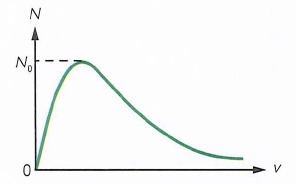
\includegraphics[width=.3\textwidth]{assets/8a0dd58e.png}
    \end{figure}
    \begin{statements}
        \task 氣體分子的平均速度增加。
        % \\The average speed of the gas molecules increases.
        \task 圖表的峰值$N_0$下降。
        % \\The peak value N$_0$ of the graph decreases.
        \task 圖表的面積保持不變。
        % \\The area under the graph remains constant.
    \end{statements}

    \begin{choices}
        \choice 只有(1)和(2)
        \choice 只有(1)和(3)
        \choice 只有(2)和(3)
        \CorrectChoice (1),(2)和(3)
    \end{choices}
}{}

\newprob{1716014582}
{
    固定質量的氣體在一個容器內。當在恆定壓強下增加氣體的溫度時,下列哪項陳述是正確的?
    % \\A fixed mass of gas is enclosed inside a container. When the temperature of the gas is increased at a constant pressure, which of the following statements is/ are correct?

    \begin{enumerate}[label=\sd]
        \item 分子更頻繁地撞擊牆壁。
              %   \par Molecules collide with the container walls more frequently.
        \item 分子受到更大的動量改變。
              %   \par Molecules experience a greater change in momentum during collisions with the container walls.
        \item 分子之間的碰撞距離變得更長。
              %   \par Molecules travel longer distances between collisions.
    \end{enumerate}


    \begin{choices}
        \choice 只有(1)和(2)
        \choice 只有(1)和(3)
        \CorrectChoice 只有(2)和(3)
        \choice (1), (2) 和 (3)
    \end{choices}
}{}

\newprob{1716014642}
{
圖中顯示固定質量的氣體其體積$V$與温度$T$的 關係。就此過程,下列哪項必定正確?
% \\A fixed mass of gas undergoes a certain process and its volume-temperature graph (V-T graph) is shown. Which of the following statements must be correct?
{\par
\centering
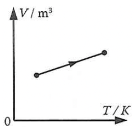
\includegraphics[width=.2\textwidth]{assets/8faae3c5.png}\par}

\begin{choices}
    \choice 該氣體並非理想氣體。
    % \The gas is not an ideal gas.
    \CorrectChoice 該氣體壓強不斷上升。
    % \\The pressure is increasing.
    \choice 氣體分子的平均動能正在減少。
    % \\The average molecular KE is decreasing.
    \choice 氣體分子之間的平均距離正在減少。
    % \\The average separation between the molecules is decreasing.
\end{choices}
}{}

\newprob{1716014667}
{
    每摩爾氦氣的質量為 4 g,每摩爾氖氣為 20 g。 若温度為$T$時,氖氣分子的方均根速率為$v$,則 同一温度下,氦氣分子的方均根速率為何?
    % \\Helium and neon have mass of \qty{4}{g.mol^{-1}} and \qty{20}{g.mol^{-1}} respectively. At a certain temperature T, the rms speed of neon molecules is v. What is the rms speed of helium molecules at the same temperature?
    \begin{choices}
        \choice $\dfrac{1}{\sqrt{5}}v$
        \choice $v$
        \CorrectChoice $\sqrt{5}v$
        \choice $5v$
    \end{choices}
}{}

\newprob{1716014699}
{
    温度 \oc{0}、壓強100 kPa的理想氣體,密度為 \qty{1.3}{kg.m^{-3}}。若壓強不變,則氣體分子在 \oc{85} 時的方均根速率是多少?
    % \\ The density of an ideal gas at \oc{0} and 100 kPa is \qty{1.3}{kg.m^{-3}}. What is the rms speed of the gas molecules at \oc{85} at the same pressure?
    \begin{choices}
        \choice \qty{320}{m.s^{-1}}
        \CorrectChoice \qty{550}{m.s^{-1}}
        \choice \qty{650}{m.s^{-1}}
        \choice \qty{880}{m.s^{-1}}
    \end{choices}
}{}

\newprob{1716014742}
{
    若壓強不變,把固定質量的理想氣體,從絕對温度$T$加熱至$2T$,則下列哪項正確?
    % \\The absolute temperature of a fixed mass of ideal gas rises from T to 2T under constant pressure. Which of the following is/are correct?

    \begin{enumerate}[label=\sd]
        \item 氣體分子的方均根速率加倍。
              %   \par The rms speed of the gas molecules is doubled.
        \item 氣體體積加倍。
              %   \par The volume of the gas is doubled.
        \item 氣體分子撞擊容器壁的頻率減至原來的 $1/\sqrt{2}$倍。
              %   \par The frequency of collision on a container wall is reduced by a factor of $\sqrt{2}$.
    \end{enumerate}
    \begin{choices}
        \CorrectChoice 只有(2)
        % \tab (2) only
        \choice 只有(3)
        % \tab (3) only
        \choice 只有(2)和(3)
        % \tab (2) and (3) only
        \choice (1), (2) 和 (3)
        % \tab (1), (2) and (3)
    \end{choices}
}{}